\documentclass{article}
\usepackage[T1]{fontenc}
\usepackage{amsmath,amsfonts,amsthm,amssymb,charter,fullpage,graphicx,inconsolata,minted,parskip}
\title{Using the Monte Carlo Process to Optimize Gasoline Inventory}
\date{November 15, 2024}
\author{Maggie Barker, Amy Lan\\MAT 301 001}
\begin{document}
    \maketitle
    \section*{Introduction}
    We are using mathematical modeling techniques to determine how much gasoline should be delivered to a chain of gasoline stations, and how often deliveries should take place, in order to minimize cost and satisfy demand. In this model, we assume that the only sources of cost are delivery and storage, that the storage cost is proportional to the amount of gasoline stored, and that the delivery cost is constant per delivery.

    We use a probabilistic submodel to approximate the daily demand. Using historical data of a particular gas station, we create a frequency table of the number of gallons demanded. From this table, we find the probability of each demand level, and build a cumulative probability table. We graph the cumulative probability histogram and approximate the cumulative probabilities with points, and then create a demand curve using cubic spline interpolation. Then we use the Monte Carlo process to find the randomized daily demand of a gas station.

    We use an algorithm to simulate the daily inventory. This algorithm accounts for periodic deliveries of gasoline, with the same time period and quantity for each delivery. We tally the cost of delivery and storage to calculate the average daily cost. To prevent running out of gas (unfilled demands), we keep track of the number of days that our inventory runs out, and the number of gallons of unfilled demands.

    We apply a range of delivery quantities and periods to simulate the average daily cost for each combination of delivery parameters. As we have two independent variables (delivery quantity and time between deliveries) and one dependent variable (average daily cost), we create a multivariable function, and we plot a 3D surface to investigate the effect of delivery parameters on cost. Our goal is to find the minimum value of this function.

    Since we assume the only sources of cost are from delivery and storage, we can reason that a low cost would be achieved by buying a small amount of gas and waiting a long time between deliveries. A minimum cost (\$0) could be achieved by never having any gas delivered, which would obviously not be conducive to a successful business operation. In fact, we would prefer to never run out of gas and be able to fulfill all demands. On the other hand, we don’t want to buy too much gasoline, or buy it too frequently, which would drive up either storage or delivery costs, or both. We would prefer a “happy medium” where we buy just enough gas to fulfill demands. So in our model, we thus modify our cost surface to cut away those combinations of quantity and frequency that result in unfilled demands. Then we find the minimum point on this new cut surface. This minimum point gives us what we are looking for: The quantity of gas to have delivered, and the frequency of delivery, that will result in minimum cost and ensure that all of our demands are fulfilled.

    As there is some randomness involved in the Monte Carlo process used in our simulation, our results are slightly different each time we run the simulation. We run the simulation many times and find the mean and standard deviation of our results. We then plot a histogram of our minimum costs to investigate the statistical distribution of our outcome.
    \pagebreak
    \section*{Methods}
    We use the table of cumulative probabilities in Table 5.8 on page 206 of the textbook (Giordano, 2014) to start building our probabilistic demand model. We perform a cubic spline interpolation from selected cumulative probability points to create a demand curve that we can use later in our Monte Carlo process. We created a MATLAB script, \texttt{cubicsplines.m}, to perform the interpolation. (Our scripts are included at the end of the document.) We get the following cubic spline polynomials:
    \begin{verbatim}
    S1: 750826.2255x^3 + 0.0000x^2 + 4924.9174x + 1000.0000, [0.00, 0.01)
    S2: -1501652.4510x^3 + 67574.3603x^2 + 4249.1738x + 1002.2525, [0.01, 0.03)
    S3: 451817.6961x^3 + -108237.9529x^2 + 9523.5432x + 949.5088, [0.03, 0.08)
    S4: -4918.9185x^3 + 1378.8346x^2 + 754.2002x + 1183.3579, [0.08, 0.20)
    S5: 2475.9884x^3 + -3058.1096x^2 + 1641.5890x + 1124.1987, [0.20, 0.40)
    S6: 140.7951x^3 + -255.8776x^2 + 520.6962x + 1273.6510, [0.40, 0.67)
    S7: 5655.7074x^3 + -11340.8515x^2 + 7947.6287x + -385.0305, [0.67, 0.85)
    S8: 11965.1108x^3 + -27429.8300x^2 + 21623.2604x + -4259.7929, [0.85, 0.93)
    S9: 382648.2595x^3 + -1061635.8148x^2 + 983434.8263x + -302421.3783, [0.93, 0.97)
    S10: -576340.2250x^3 + 1729020.6751x^2 + -1723501.9689x + 572821.5188, [0.97, 1.00)\end{verbatim}
    In Figure \ref{fig:cubicsplines} on page \pageref{fig:cubicsplines}, we plot the cumulative probability points with the cubic spline polynomials to visually confirm that the splines are a good fit.
    \begin{figure}[p]
        \centering
        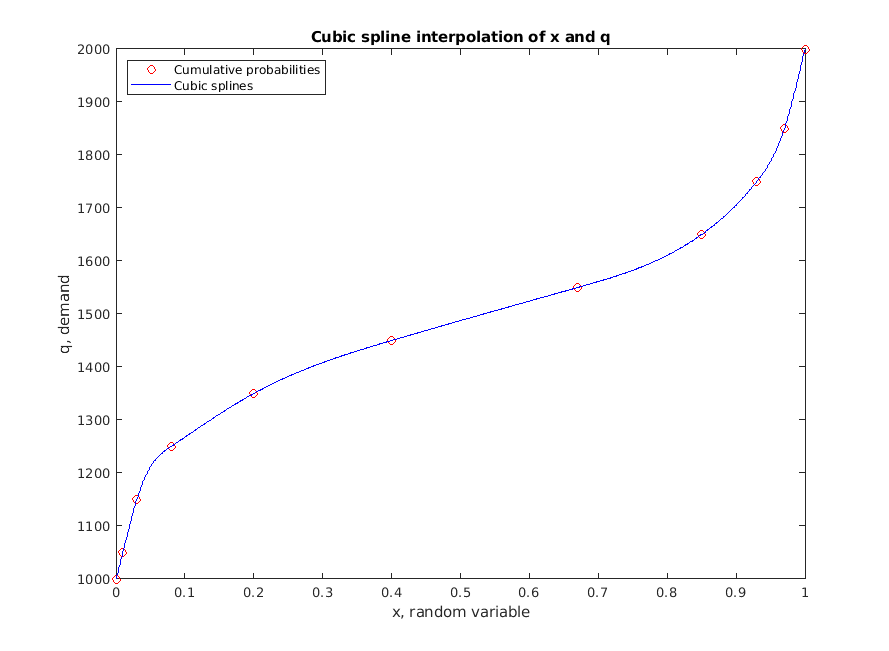
\includegraphics[width=\textwidth]{cubicsplines.png}
        \caption{Cumulative probability plot, with cubic spline interpolating polynomials superimposed.}
        \label{fig:cubicsplines}
    \end{figure}
    Then we use another MATLAB script, \texttt{demand.m}, to evaluate our piecewise polynomial function for each random number from 0 to 1. We hardcoded the coefficients that resulted from \texttt{cubicsplines.m} to avoid recalculating the cubic splines every time we run the simulation. Our \texttt{demand} function has the following signature:
    \begin{minted}{matlab}
    function q = demand(x)
    % Calculates demand based on a random variable x
    % x must be a scalar in the interval [0, 1]
    \end{minted}
    In another MATLAB script, \texttt{inventory.m}, which functions as the core of our model, we perform the actual simulation. Our inventory function has the following signature:
    \begin{minted}[breaklines]{matlab}
    function [c, L, D] = inventory(Q, T, d, s, N)
    % Simulates inventory by Monte Carlo method
    % Q: Delivery quantity of gasoline in gallons
    % T: Time between deliveries in days
    % d: Delivery cost in dollars per delivery
    % s: Storage cost per gallon per day
    % N: Number of days to run the simulation
    % Returns [average daily cost, number of days with unfilled demands, amount of unfilled demand in gallons]
    \end{minted}
    We create variables as follows:\\
    \texttt{K}: Number of days remaining in the simulation\\
    \texttt{I}: Current inventory in gallons\\
    \texttt{C}: Total running cost\\
    \texttt{L}: Number of days with unfilled demands\\
    \texttt{D}: Amount of unfilled demands in gallons\\
    \texttt{flag}: An indicator used to terminate the algorithm\\

    \pagebreak
    We initially set \texttt{K} to equal \texttt{N}, the number of days to run the simulation, and we set \texttt{I}, \texttt{C}, \texttt{L}, \texttt{D}, and \texttt{flag} to equal \texttt{0} initially. Then we use a \texttt{while} loop to run the simulation until we are ready to terminate it. We begin the cycle with a delivery, so we increase the inventory \texttt{I} by the quantity \texttt{Q} that was delivered, and we increase the total cost \texttt{C} by the delivery cost \texttt{d}. We check to see if the simulation will stop before our next delivery, and if so, we set the termination \texttt{flag} to \texttt{1} and we reduce the inventory cycle time \texttt{T} to be the number of days left in the simulation.

    Then we use a \texttt{for} loop to iterate over the \texttt{T} days, which will either be the number of days between deliveries, or the number of days until the simulation ends, whichever is least. We generate a random number between \texttt{0} and \texttt{1}, and we call our \texttt{demand} function in \texttt{demand.m} to find the demand from our random variable using the piecewise spline polynomial. If our demand is more than our remaining inventory, we increment the counter \texttt{L} to keep track of the number of days that we have unfilled demands. We also increase \texttt{D} by the deficit to keep track of the number of gallons of unfilled demands. We will use this information later. Then we deduct the demand from the inventory. If we have completely depleted our inventory, we set our inventory to zero because we cannot have negative inventory. If we have any inventory remaining, we need to store it, incurring storage costs. So we increase our total cost \texttt{C} by the storage cost \texttt{I*s}, which is the amount of inventory in gallons multiplied by the storage cost per gallon. Then we reduce the number of days remaining, and the \texttt{for} loop repeats for the next day in the inventory cycle. Once the inventory cycle (or simulation) is over, the \texttt{while} loop checks if the termination \texttt{flag} has been set to \texttt{1}, indicating that the simulation should end. If not, we get another delivery and repeat the process until termination.

    Once we terminate the simulation, we calculate the average daily cost by dividing the total running cost by the number of days simulated, and we return this value, along with the number of days of unfilled demands and the number of gallons unfilled.

    Now we use another MATLAB script, \texttt{optimize.m}, to run our inventory script for a range of different delivery quantities and frequencies. Our \texttt{optimize} function has the following signature:
    \begin{minted}[breaklines]{matlab}
    function [min_cost, min_Q, min_T] = optimize(d, s, N, plots)
    % Finds optimum delivery quantity in gallons and time between deliveries in days to minimize average daily cost
    % d: Delivery cost in dollars per delivery
    % s: Storage cost per gallon per day
    % N: Number of days to run the simulation
    % plots: Whether to show surface plots or not
    % Returns [minimum cost, quantity, time]
    \end{minted}
    We need to make some assumptions to limit our ranges of \texttt{Q} and \texttt{T} (delivery quantity and period, respectively). Let us assume that the most frequently we should expect deliveries is every three days, and the least frequently is every thirty days. We only consider whether a delivery takes place during a given day or not, and fractional days are irrelevant, so the number of days between deliveries is an integer between 3 and 30. Considering that the daily demand ranges from 1,000 to 2,000 gallons, we want to find the extreme quantities that we should consider  for delivery. At a minimum, if we have gas delivered every three days, and we expect the lowest demand each day, we would need 3,000 gallons delivered each time. At a maximum, if we have gas delivered every thirty days, and we expect the highest demand each day, we would need 60,000 gallons delivered each time. To make our cost surface smoother, we should have a small step between delivery quantities, but to make our code faster, we should have a large step. After trial and error, we found that the compromise step value of 500 works well. Thus, we have the following ranges of values to test:
    \begin{minted}{matlab}
    Q = 3000:500:60000;
    T = 3:1:30;
    \end{minted}

    \pagebreak
    We create a large matrix (115 x 28) to hold the average daily cost for each value of \texttt{Q} and \texttt{T}. We also create a matrix of the same size for the number of days with unfilled demands, and a matrix for the number of gallons unfilled. Finally, we create a fourth matrix that will contain the average daily cost, but with those combinations of \texttt{Q} and \texttt{T} that result in unfilled demands removed. We use the following double \texttt{for} loop to run the simulation over all combinations of \texttt{Q} and \texttt{T} and populate our matrices:
    \begin{minted}[breaklines]{matlab}
    for i = 1:length(Q)
        for j = 1:length(T)
            [cost(i, j) unfilled_days(i, j) unfilled_gallons(i, j)] = inventory(Q(i), T(j), d, s, N);
            if unfilled_days(i, j) > 0
                cost_remove_unfilled(i, j) = NaN;
            else
                cost_remove_unfilled(i, j) = cost(i, j);
            end
        end
    end
    \end{minted}

    Then we create four surface plots, all with quantity and period of deliveries as the independent variables, with the following dependent variables:
    \begin{itemize}
        \item Minimum average daily cost,
        \item Days with unfilled demands,
        \item Gallons of unfilled demands, and
        \item Minimum average daily cost (unfilled demands removed)
    \end{itemize}

    Next, we use the following code to find our minimum daily cost (with no unfilled demands) and with which combination of \texttt{Q} and \texttt{T} it occurs:

    \begin{minted}{matlab}
    min_cost = min(min(cost_remove_unfilled));
    [min_i min_j] = find(cost_remove_unfilled == min(min(cost_remove_unfilled)));
    min_Q = Q(min_i);
    min_T = T(min_j);
    \end{minted}

    We return the coordinates \texttt{min\_cost}, \texttt{min\_Q}, and \texttt{min\_T}, which represent the minimum value of the cost function and the point where it occurs.

    We use a simple script to perform a single simulation, \texttt{singlesimulation.m}. However, there are still two questions we have not answered. How much does each delivery cost? What is our storage cost per gallon? We have assumed these to be constant, but we have not specified what values these constants should have. We used the information given in Project 2 on page 213 (Giordano, 2014) to find reasonable values of \$500 per delivery and \$0.001 per gallon stored. We also decided to run the simulation for 365 days at a time. Finally, we use the MATLAB stopwatch functions \texttt{tic} and \texttt{toc} to time the run of our algorithm.

    \begin{minted}[breaklines]{matlab}
    tic
    d = 500; % Delivery cost
    s = 0.001; % Storage cost
    N = 365; % Number of days
    clf
    [min_cost min_Q min_T] = optimize(500, 0.001, 365, true);
    fprintf("Delivery cost: %d\nStorage cost: %.3f\nDays simulated: %d\nMinimum average daily cost: $%.2f\nDelivery quantity: %d\nTime between deliveries: %d\n", d, s, N, min_cost, min_Q, min_T);
    toc
    \end{minted}

    As addressed earlier, there is some variation in our results every time we run the algorithm, so we want to find an average of multiple runs. We do this in our MATLAB script \texttt{multiplesimulations.m}. We want to avoid making surface plots for every single run, so we have an argument in our optimize function to allow us to suppress the plots.  We implemented a stopwatch and a progress indicator while the simulations are running, since it can take quite a while with many iterations. Then we output our results in a matrix, perform a quick statistical summary with the MATLAB \texttt{summary} command, and draw a histogram of our minimum average daily costs to visualize the distribution of our costs, which we might expect to be normal.

    Finally, our average values of our minimum average daily cost, and the average values of \texttt{Q} and \texttt{T}, give us a best estimate of how much gasoline we should have delivered and how often to schedule deliveries. The standard deviations of these values give us an idea of the precision of our simulation.
    \section*{Results}
    We are running the \texttt{singlesimulation.m} script to perform a single simulation and optimization. Our output is as follows:

    \begin{verbatim}
    Delivery cost: 500
    Storage cost: 0.001
    Days simulated: 365
    Minimum average daily cost: $40.52
    Delivery quantity: 38000
    Time between deliveries: 25
    Elapsed time is 1.573916 seconds.\end{verbatim}

    We will discuss this output after we take a look at our surface plots.

    Our surface plots are as follows:\\
    \begin{itemize}
        \item Figure \ref{fig:surface1} (page \pageref{fig:surface1}): Minimum average daily cost,
        \item Figures \ref{fig:surface2} (page \pageref{fig:surface2}) and \ref{fig:surface21} (page \pageref{fig:surface21}): Days with unfilled demands,
        \item Figure \ref{fig:surface3} (page \pageref{fig:surface3}): Gallons of unfilled demands, and
        \item Figure \ref{fig:surface4} (page \pageref{fig:surface4}): Minimum average daily cost (unfilled demands removed)
    \end{itemize}

    In Figure \ref{fig:surface1}, we can see that the highest average daily cost (approximately \$3,600) is incurred when deliveries take place every three days, and when 60,000 gallons are delivered each time. The dark blue flat region of the surface indicates a low average daily cost. This surface disregards the situation in which the station does not have enough gasoline to satisfy demand.

    In Figure \ref{fig:surface2}, we can see that for lower delivery quantities and longer delivery periods, there will be days that the station does not have enough gasoline to satisfy demand. In this particular instance, when 3,000 gallons of gasoline are delivered every 30 days, the station will have unfilled demands 342 out of 365 days (94\%), which is clearly unacceptable. Interestingly, there is a straight line in the $Q-T$ plane, on one side of which, all demands are fulfilled, and on the other side, there are unfilled demands. We now rotate the plot so that the viewing angle is "top down", to get a better look at the $Q-T$ plane in Figure \ref{fig:surface21}.

    In Figure \ref{fig:surface21}, we see more clearly the dividing line between fulfilled demands (the dark blue region) and unfilled demands (the multicolored region). This dividing line approximately follows the linear equation $Q = 1500T$. This makes sense, since the daily demand is simulated to be between 1,000 and 2,000 gallons per day, with an average demand near 1,500 gallons per day, as seen in Figure \ref{fig:cubicsplines} on page \pageref{fig:cubicsplines}.

    Figure \ref{fig:surface3} looks similar to Figure \ref{fig:surface2}, but it is showing the unfilled demand in \emph{gallons} rather than the number of days with unfilled demands. Figure \ref{fig:surface2} is a graphical indicator of the variable \texttt{L} in the algorithm, while Figure \ref{fig:surface3} is an indicator of \texttt{D}. As may be expected, these graphs have a similar shape but a different scale.

    In Figure \ref{fig:surface4}, those combinations of delivery quantity and period that result in unfilled demands (the multicolored region of Figure \ref{fig:surface21}) have been cut away, leaving only those parts of the surface where all demands are fulfilled. Our goal is to find the minimum average daily cost with no unfilled demands, and that is represented by the lowest point on the surface in Figure \ref{fig:surface4}.

    \begin{figure}[h]
        \centering
        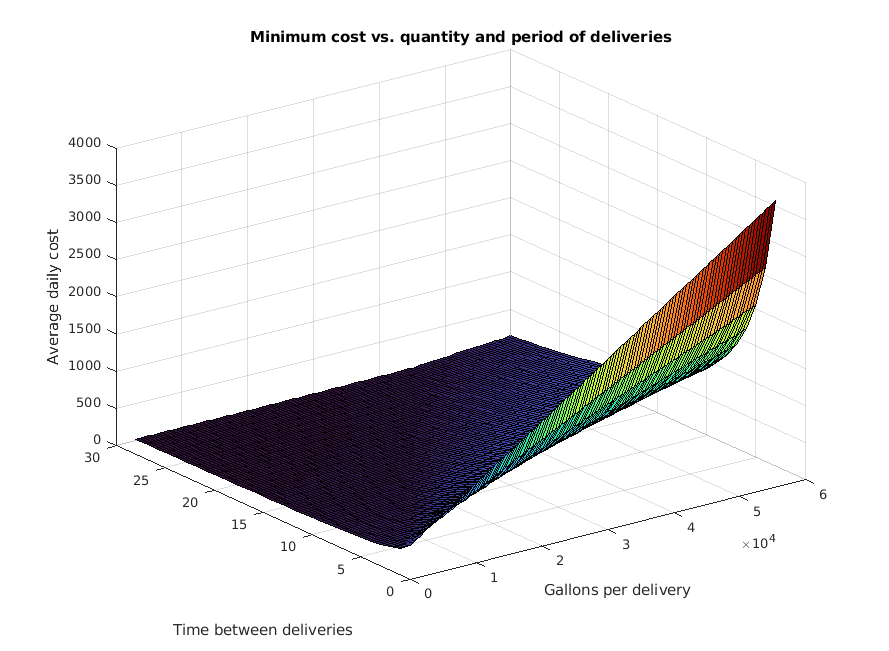
\includegraphics[width=\textwidth]{surface1.png}
        \caption{Minimum average daily cost vs. delivery quantity and period.}
        \label{fig:surface1}
    \end{figure}

    \begin{figure}[p]
        \centering
        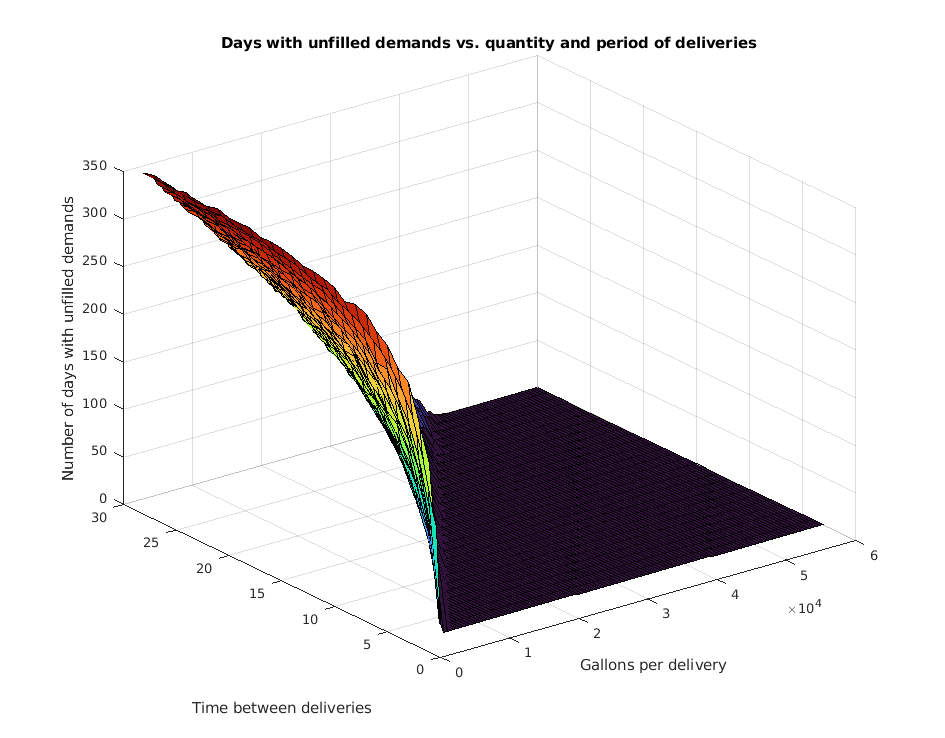
\includegraphics[width=\textwidth]{surface2.png}
        \caption{Number of days with unfilled demands vs. delivery quantity and period.}
        \label{fig:surface2}
    \end{figure}

    \begin{figure}[p]
        \centering
        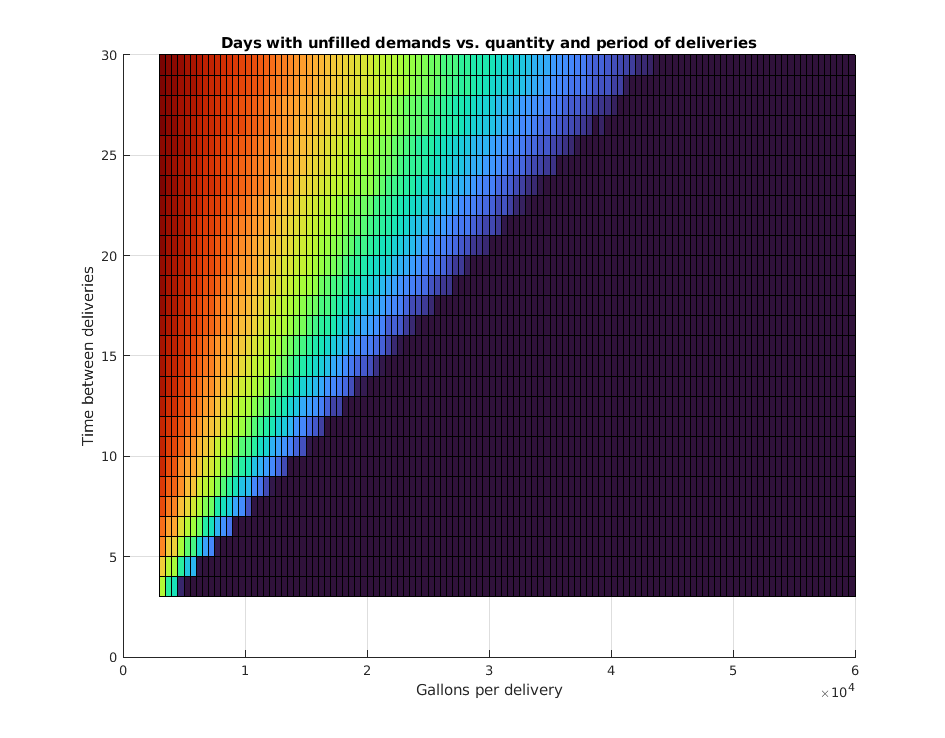
\includegraphics[width=\textwidth]{surface2.1.png}
        \caption{Number of days with unfilled demands vs. delivery quantity and period. This is the same surface as in Figure \ref{fig:surface2}, with a different viewing aspect.}
        \label{fig:surface21}
    \end{figure}

    \begin{figure}[p]
        \centering
        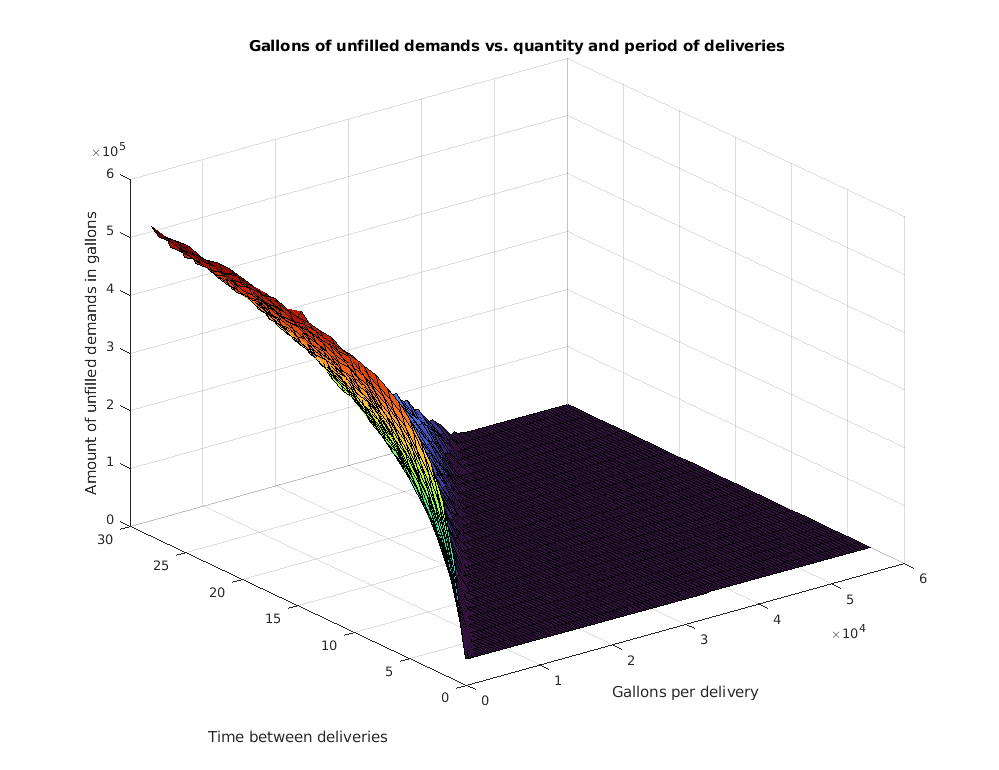
\includegraphics[width=\textwidth]{surface3.png}
        \caption{Gallons of unfilled demands vs. delivery quantity and period.}
        \label{fig:surface3}
    \end{figure}

    \begin{figure}[p]
        \centering
        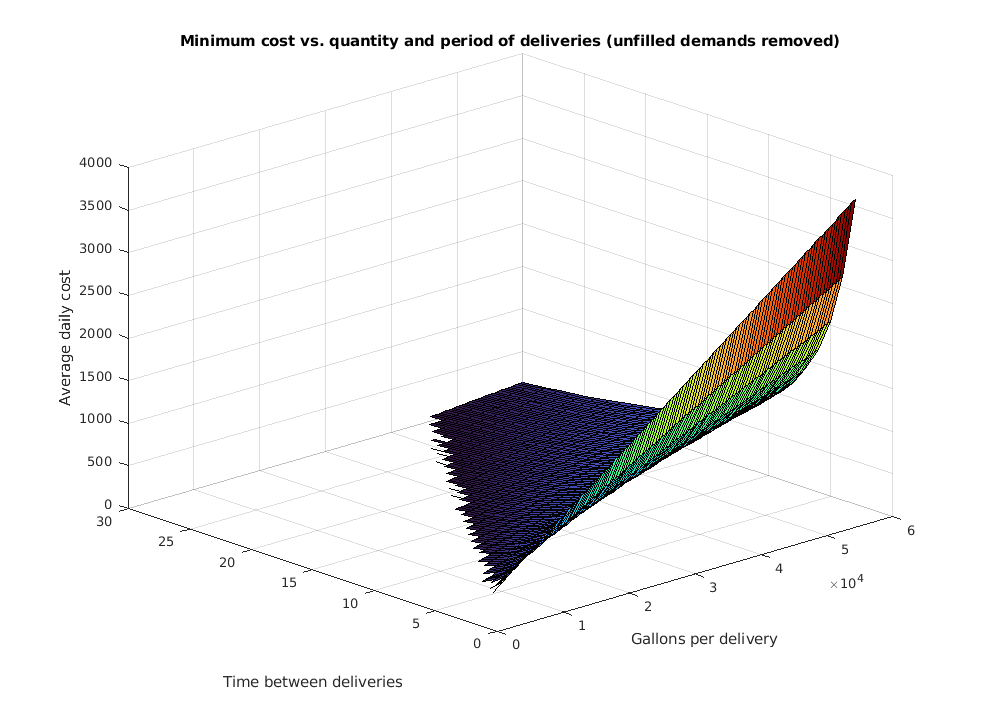
\includegraphics[width=\textwidth]{surface4.png}
        \caption{Minimum average daily cost vs. delivery quantity and period. Combinations of delivery quantity and period that result in unfilled demands have been cut away.}
        \label{fig:surface4}
    \end{figure}

    \clearpage

    We return to the output from our script to analyze it further.

    \begin{verbatim}
    Delivery cost: 500
    Storage cost: 0.001
    Days simulated: 365
    Minimum average daily cost: $40.52
    Delivery quantity: 38000
    Time between deliveries: 25
    Elapsed time is 1.573916 seconds.\end{verbatim}

    The delivery cost, storage cost, and days simulated are constants that we specified. The elapsed time shows that our simulation takes approximately 1.6 seconds to run, which is an important consideration when we want to run multiple simulations. The key insight given here is in lines 4 through 6. This shows that the minimum average daily cost with no unfilled demands is \$40.52 (\texttt{min\_cost}), and this occurs when deliveries of 38,000 gallons (\texttt{`min\_Q`}) take place every 25 days (\texttt{min\_T}). That is excellent information, but we still have one major concern. Every time we run the simulation and optimization process, we get a slightly different result. This variation stems from the randomness in the Monte Carlo demand simulation. The plots look roughly the same, so we will only consider the changes in numerical output. Here are the outputs from eight additional runs:

    \begin{verbatim}
    Minimum average daily cost: $40.66
    Delivery quantity: 39000
    Time between deliveries: 26

    Minimum average daily cost: $41.16
    Delivery quantity: 44000
    Time between deliveries: 29

    Minimum average daily cost: $40.72
    Delivery quantity: 34500
    Time between deliveries: 23

    Minimum average daily cost: $41.07
    Delivery quantity: 43000
    Time between deliveries: 29

    Minimum average daily cost: $40.63
    Delivery quantity: 39000
    Time between deliveries: 26

    Minimum average daily cost: $40.89
    Delivery quantity: 44500
    Time between deliveries: 30

    Minimum average daily cost: $40.50
    Delivery quantity: 41500
    Time between deliveries: 28

    Minimum average daily cost: $41.37
    Delivery quantity: 44500
    Time between deliveries: 30\end{verbatim}
    \pagebreak

    As can be seen, the variation is not very large, since the minimum average daily cost remains roughly around \$41. The delivery quantities are approximately 35,000-45,000 gallons, and the delivery periods are around 23-30 days.

    To get a better idea of the variation at play, we now run our \texttt{multiplesimulations.m} script to easily perform 1,000 runs and collect the data. Considering that one simulation and optimization takes around 1.6 seconds to perform, we figure this will take quite some time. To have a visual indication that the script is still running, we output a message after every simulation, along with a progress indicator.

    \begin{verbatim}
    Performing simulation 1 of 1000 (0.10%)...
    Performing simulation 2 of 1000 (0.20%)...
    Performing simulation 3 of 1000 (0.30%)...
    Performing simulation 4 of 1000 (0.40%)...
    Performing simulation 5 of 1000 (0.50%)...
    Performing simulation 6 of 1000 (0.60%)...
    Performing simulation 7 of 1000 (0.70%)...
    Performing simulation 8 of 1000 (0.80%)...
    Performing simulation 9 of 1000 (0.90%)...
    Performing simulation 10 of 1000 (1.00%)...\end{verbatim}

    After about 24 minutes, the final output is as follows, where the first column is minimum average daily cost (\texttt{min\_cost}), the second column is delivery quantity (\texttt{min\_Q}), and the third column is delivery period (\texttt{min\_T}):

    \begin{verbatim}
    41.58      34000.00         23.00
    40.46      38500.00         26.00
    40.66      38500.00         26.00
    40.62      33000.00         22.00
    42.56      43500.00         29.00
    41.95      36000.00         24.00
    41.70      37500.00         25.00
    40.96      34500.00         23.00
    40.30      34500.00         23.00
    41.40      41500.00         28.00
    ...
    40.73      33000.00         22.00
    39.89      38500.00         26.00
    40.34      39000.00         26.00
    40.29      36000.00         24.00
    40.46      40000.00         27.00


    results: 1000×3 double

    NumMissing          0               0            0
    Min             39.12        28000.00        19.00
    Median          41.14        38000.00        25.00
    Max             43.96        45500.00        30.00
    Mean            41.19        38310.50        25.63
    Std              0.81         3914.23         2.63

    Elapsed time is 1453.711439 seconds.\end{verbatim}
    \pagebreak
    Here we see the mean of the minimum average daily costs (N = 1,000) is \$41.19, where the mean gallons per delivery is 38,310.50 gallons, and the mean days between deliveries is 25.63. Thus, it appears that the cost can be minimized by ordering around 38,000-39,000 gallons every 25-26 days, which is in close agreement with our initial run above. We note that the standard deviation of the minimum average daily cost is \$0.81, the standard deviation of gallons per delivery is 3,914.23 gallons, and the standard deviation of time between deliveries is 2.63 days. We also note that the mean (\$41.19) and median (\$41.14) of the minimum average daily cost are approximately equal, indicating that the distribution is not significantly skewed. Finally, we look at a histogram of minimum average daily cost (Figure \ref{fig:histogram}) to see that it is approximately normally distributed.

    \begin{figure}[h]
        \centering
        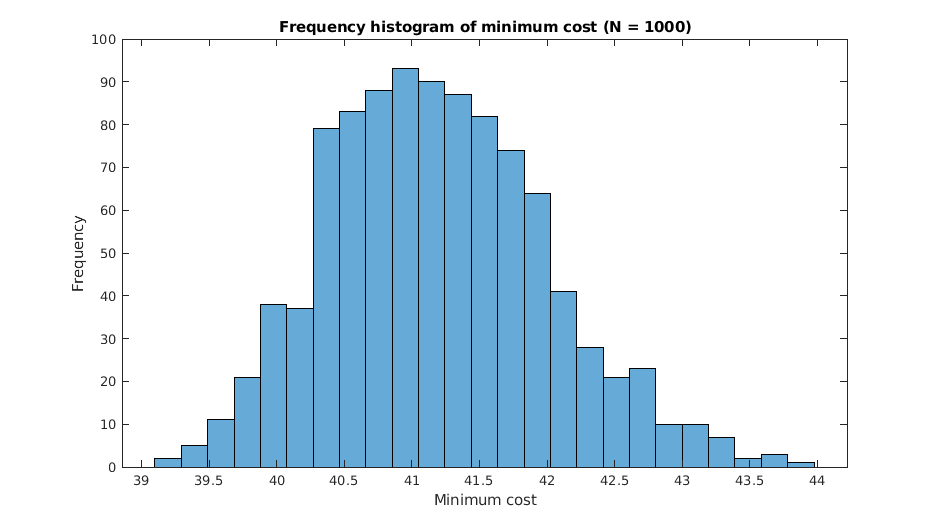
\includegraphics[width=\textwidth]{histogram.png}
        \caption{Frequency histogram of minimum average daily cost (N = 1,000). This reveals a symmetric distribution of minimum average daily cost that is approximately normal, with the mode in the bin from \$40.855 to \$41.05.}
        \label{fig:histogram}
    \end{figure}
    \pagebreak
    \section*{Conclusion}
    \pagebreak
    \section*{Scripts}
    Our MATLAB code is listed here, and it is downloadable from the following URL:\\
    https://github.com/marautbar/mat-301-inventory-project
    \subsection*{cubicsplines.m}
    \inputminted[linenos,breaklines]{matlab}{cubicsplines.m}
    \subsection*{demand.m}
    \inputminted[linenos,breaklines]{matlab}{demand.m}
    \subsection*{inventory.m}
    \inputminted[linenos,breaklines]{matlab}{inventory.m}
    \subsection*{optimize.m}
    \inputminted[linenos,breaklines]{matlab}{optimize.m}
    \subsection*{singlesimulation.m}
    \inputminted[linenos,breaklines]{matlab}{singlesimulation.m}
    \subsection*{multiplesimulations.m}
    \inputminted[linenos,breaklines]{matlab}{multiplesimulations.m}
    \pagebreak
    \section*{References}
    Giordano, F., Fox, W., Horton, S. \emph{A First Course in Mathematical Modeling, Fifth Edition.} Cengage Learning. 2014.
\end{document}